\chapter{LUX Post-Run 04 Calibration Campaign}
After the LUX Run4 WIMP-search was completed in June of 2016, the response of the detector was exercised using ER and NR calibration sources. The usual ER calibrations of krypton-83m\cite{lux_kr1,lux_kr2} and tritiated methane (CH$_3$T)\cite{lux_tritium} were performed, along with NR calibrations using the deuterium-deuterium (DD) neutron generator\cite{lux_dd1,lux_dd2}. In addition to these standard calibrations, there were additional techniques and sources used which were novel to the LUX detector. 

The first novel calibration performed was a modification to the DD NR calibration. The rest of these new calibrations were to the ER response and will be the primary focus of this chapter, but we will pause here briefly to discuss the DD calibrations. The NR response of the LUX detector was measured using a beam of neutrons which was directed into the cryostat. These neutrons were generated using a commercially available DD generated, and were collimated using a gas filled conduit which was suspended in the water tank. Because the neutrons entering the detector have a known energy and direction, it is then possible to calculate the precise recoil energy of a neutron from the beam scattering off of a xenon nucleus, assuming the scattering angle is known. The calculation is the same for neutron-nucleus scattering as for WIMP-nucleus scattering:
\begin{equation}
E_R=\frac{E_nr}{2}[1-\cos(\theta)],
\end{equation}
where $\theta$ is the scattering angle in the center of mass frame, and $r=4M_AM_n/(M_A+M_n)^2$. The scattering angle in the lab frame can be easily measured for events where the scattered neutron interacts with a second xenon atom before exiting the detector, and for large nuclei such as xenon, the approximation $\theta_{CM}\approx \theta_{LF}$ can be made. The result of this procedure is a continuous NR recoil spectrum where the energy of each event is precisely known. These events will be located along the beam line, so will be at roughly the same drift time. By moving the conduit up and down, the detector NR response as a function of drift time can be mapped out.\cite{lux_dd1,lux_dd2}
\begin{figure}[h!]
\centering
\begin{subfigure}{0.5\textwidth}
  \centering
  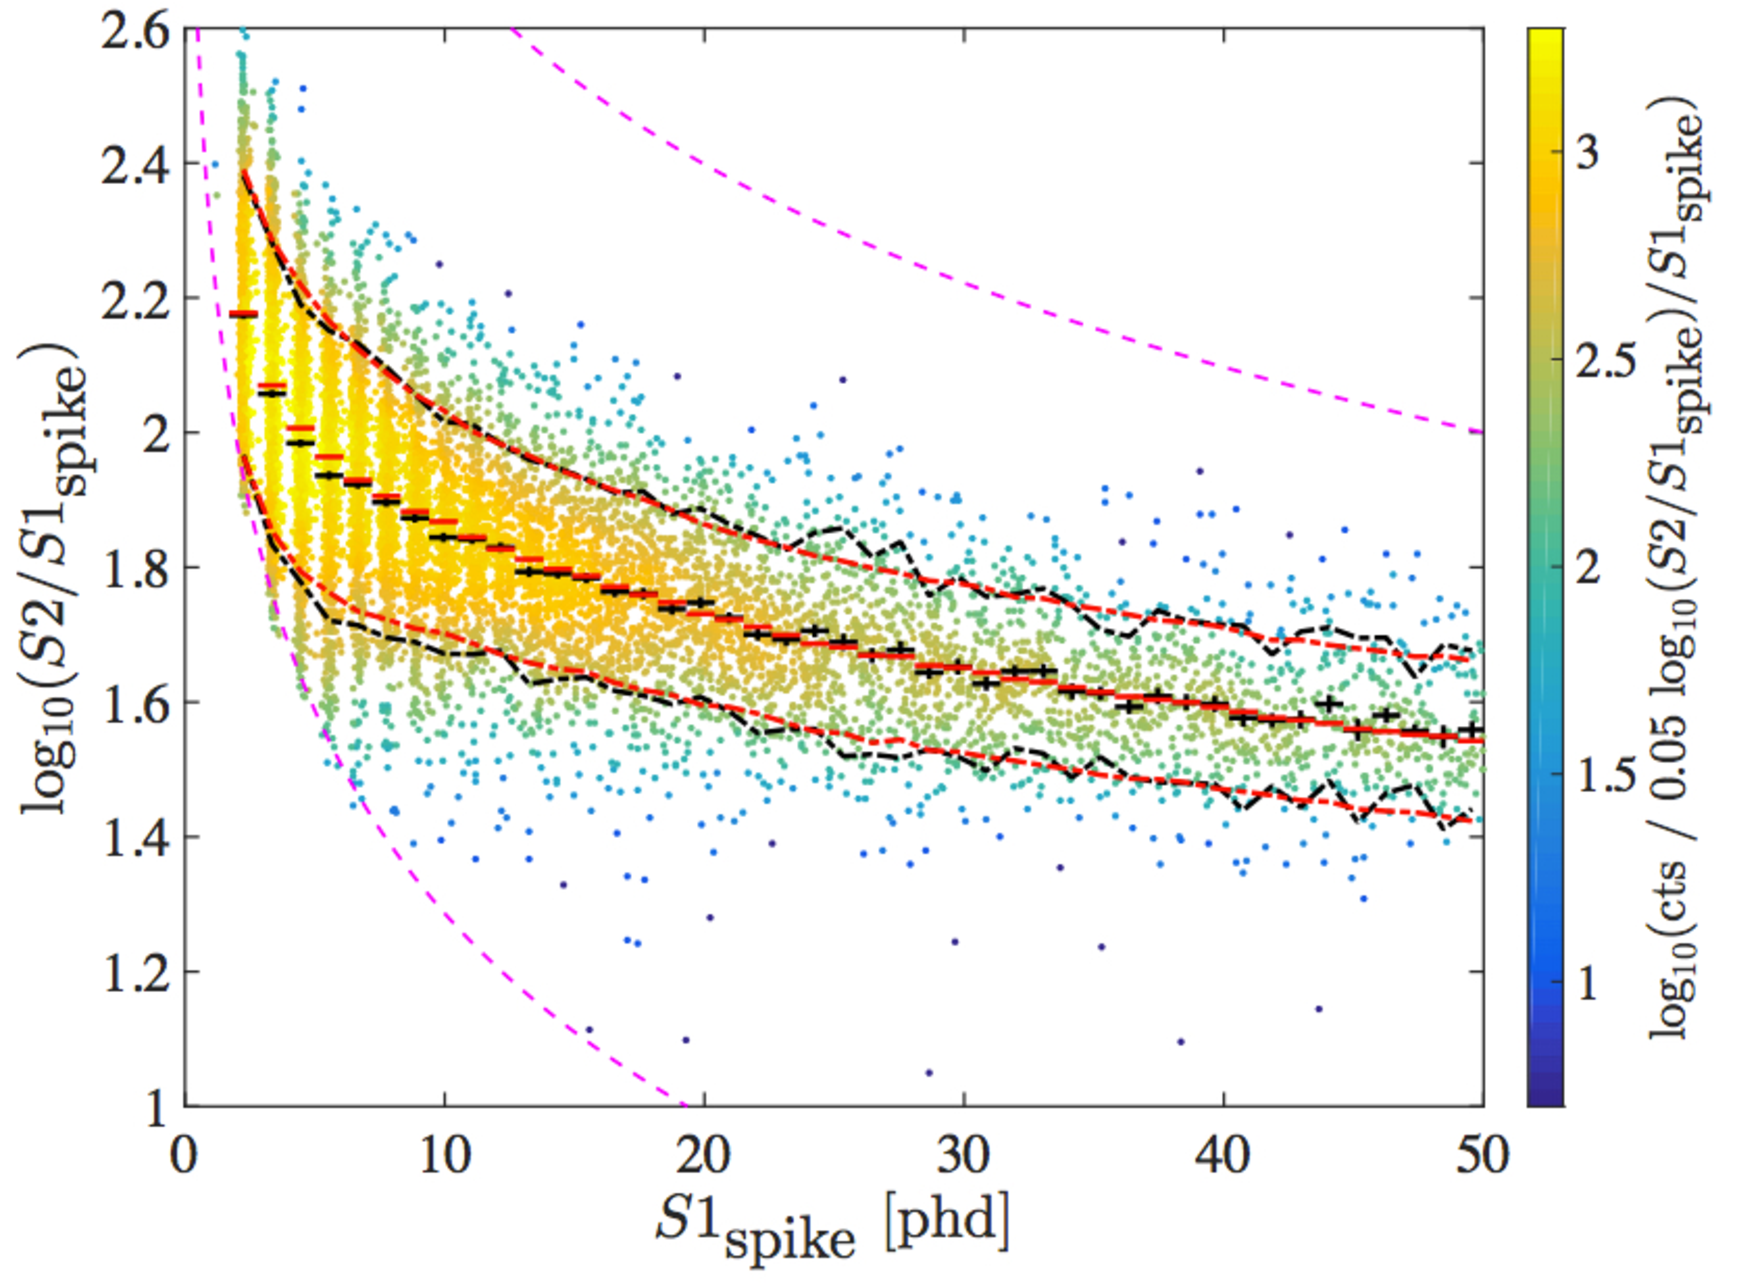
\includegraphics[width=\textwidth]{Figures/DDband.pdf}
  %\label{}
\end{subfigure}%
\begin{subfigure}{0.5\textwidth}
  \centering
  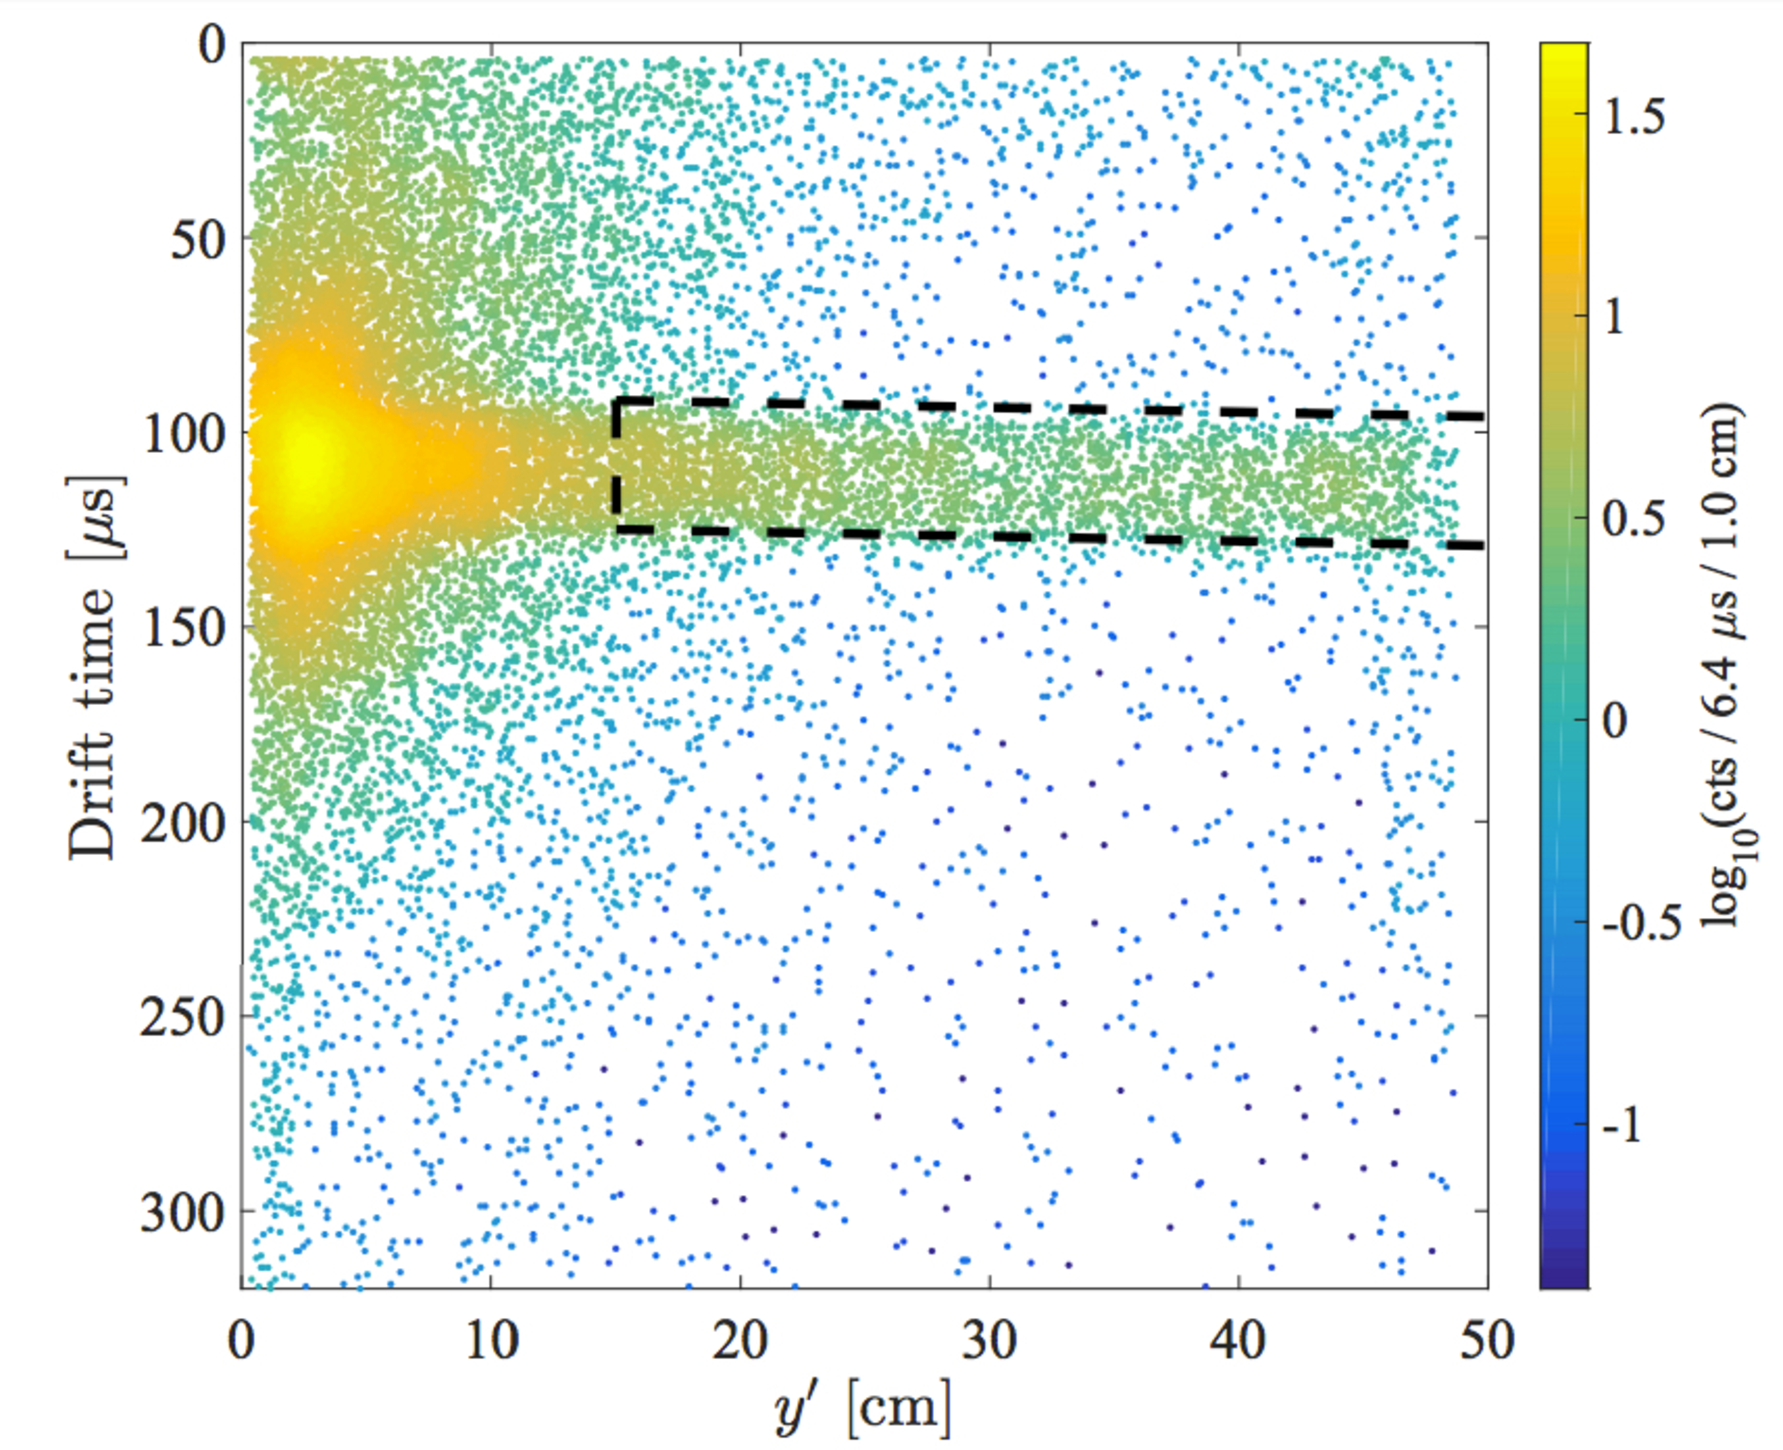
\includegraphics[width=\textwidth]{Figures/DDbeam.pdf}
  %\label{fig:intlin}
\end{subfigure}
\caption{Plots of the measured neutron beam line (left) and the NR recoil band (right) from a previous LUX D-D calibration. The $y'$ coordinate in the beam line plot is a transformation of the standard LUX $x$ and $y$ coordinates, such that it it measures the horizontal distance along the beam line. The NR recoil band plot shows the continuous nature of the recoil spectrum. Figures taken from \cite{lux_dd2} }
\label{fig:ddplot}
\end{figure}

The novel modification to the DD calibration in the post-run 04 campaign was to first scatter the neutrons off of a D$_2$O target before sending them into the conduit. The only neutrons of a single, known, scattering angle will pass through the conduit, so this procedure effectively converts the 2.45 MeV mono-energetic neutron source to a 272 keV mono-energetic neutron source. The main portion of the post-Run4 DD campaign ended on August 7$^{th}$, although there was a final brief period of testing between August 22$^{nd}$ and 23$^{rd}$.\cite{lux_dd1}


On August 9$^{th}$, $^{131m}$Xe became the first of the non-standard, post-Run4 ER sources to be injected. The 12 day half life of this source meant that all subsequent sources in the month long campaign have the $^{131m}$Xe line as a background. The $^{131m}$Xe line is sufficiently separated in energy from most of the other sources, so that this background will not have a significant effect. However, the $^{131m}$Xe line, which lies at 164 keV, is only 8 keV above the $^{14}$C Q value of 156 keV and so obscures the highest-energy portion of the $^{14}C$ beta spectrum.

The tritium calibration was started on the 18$^{th}$, and the second new ER source, $^{14}$C was injected five days later on the 23$^{rd}$. Both of these sources rely on the injection of radio-labelled methane and are purified out by the LUX getter with a time constant of about 10 hours. This means that the tritium will have been reduced by about 12 e-folds, or a factor of 150,000, by the time the $^{14}$C was injected. Since the amount of of tritium events in this injection was about 1 million, there should be an overlap of <10 events in the $^{14}$C injection.

The next source injected was radon-220. There were two injections, with peak activities of about 50 Hz on the 27$^{th}$ and on 29$^{th}$. Radon-220 is part of the thoron-232 decay chain, which ends with the stable lead-208. The transition time from $^{220}$Rn to $^{208}$Pb is dominated by the $\beta^-$ decay of $^{212}$Pb to $^{212}$Bi, which has a half life of about 10.6 hours. 

A 70 Hz injection of $^{37}$Ar took place on the 31$^{st}$, about 3 days after the second radon-220 injection. This meant that there was about 1 Hz of $^{212}$Pb remaining in the detector. The most common and most energetic $^{37}$Ar decay will deposit 2.8 keV into the xenon via x-ray. This is low energy means that the $^{37}$Ar decays will be well separated from the MeV-level alphas and betas of $^{212}$Pb and its daughters. The high rate and 35 day half life of the injected $^{37}$Ar meant that this was the final injection performed in the post-Run4 campaign, and was in fact the last physics data collected by the LUX detectors.

The rest of this chapter will focus on the $^{131m}$Xe, $^{37}$Ar, and $^{14}$C sources. We will also present a review $^{83m}$Kr and $^{3}$H. This particular suite of sources is exciting in the fact that it includes two continuous beta spectra, which can be used to map out xenon ER yields from 140 keV down to threshold, as well as three ER lines that can be used to correct for position dependent detector efficiency and examine systematic pathologies.
\begin{figure}[h!]
\centering
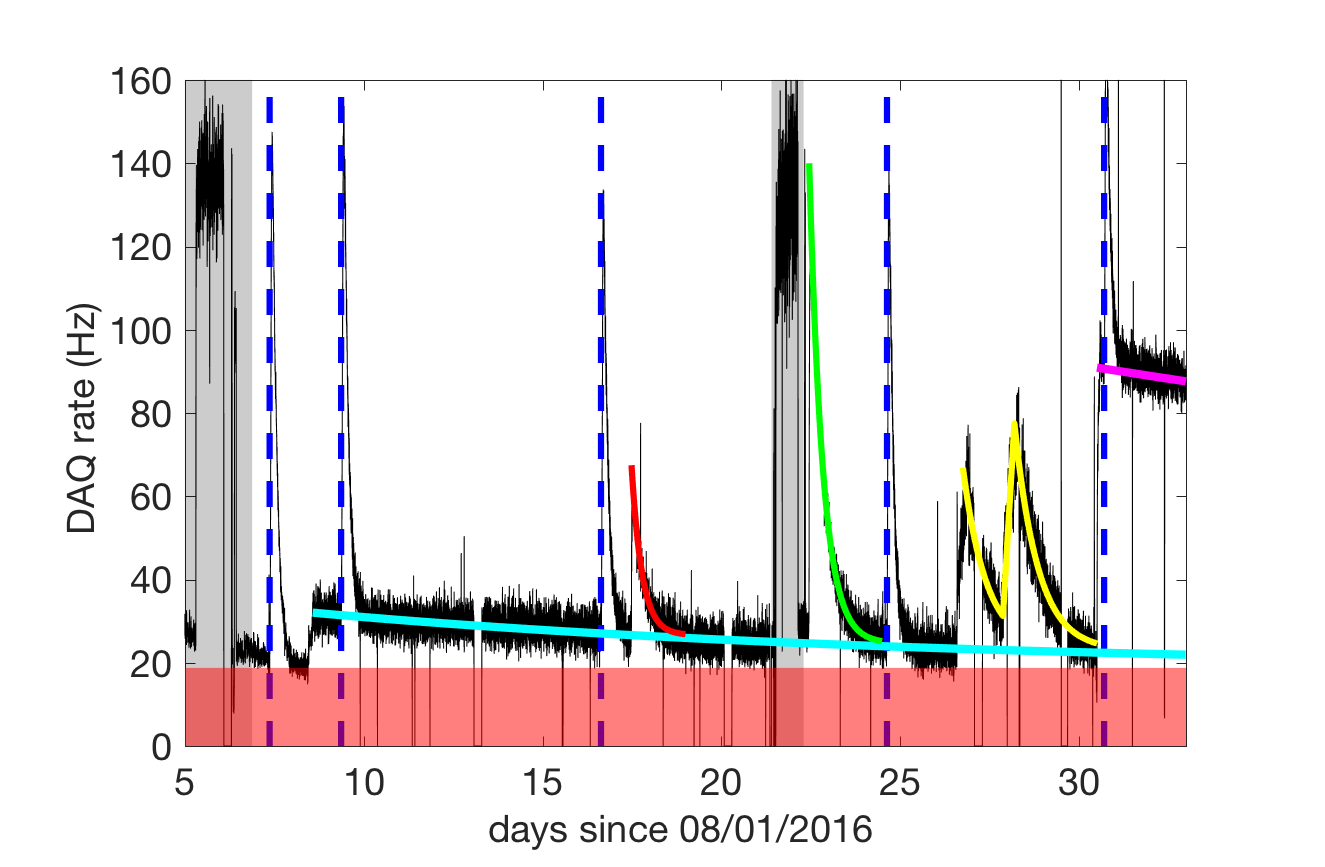
\includegraphics[width=\textwidth]{Figures/post_Run4_DAQrate.eps}
\caption{The black line shows the DAQ rate for the post-run04 injection campaign. The red shaded region shows the constant baseline, while the grey shaded regions show the DD NR-calibration campaign. The vertical dashed blue lines show the times of standard $^{83}$Kr$_m$ injections. The cyan, red, green, yellow, and magenta lines trace the $^{131m}$Xe, $^{3}$H, $^{14}$C, $^{220}$Rn, and $^{37}$Ar activities, respectively.} 
\label{fig:DAQrate}
\end{figure}

\section{Data Selection}
There were several preliminary data selection cuts applied to isolate the $^{37}$Ar K-capture, $^{131m}$Xe, $^{83m}$Kr, $^{3}$H, and $^{14}$C events. The time interval which these events were drawn from August 17 until September 3. In figure \ref{fig:DAQrate} this corresponds to the third krypton injection at T=16.6 days, until the end of data taking. The periods of DD generator and $^{220}$Rn activity were excluded (from T=21.4 to 22.3 days and T= 26.8 to 30.5 days, respectively). There was also a period of time after the $^{14}$C calibration, from T=24.5 to 26.8 days, where one of the PMT's was misbehaving. This time period, which included the fourth krypton injection, was also rejected.

\section{Argon 37}
Argon-37 provides three useful low-energy ER calibration lines. It decays through electron capture to $^{37}$Cl with a half life of 35 days. The long half life, combined with the fact that argon is chemically inert means that once injected, it will be on the order of a year before it has been sufficiently removed. That being the case, it was only injected immediately prior to LUX decommissioning.\cite{ar371,pixey_ar37}

The $^{37}$Ar source was produced through stimulated $\alpha$ emission of a $^{40}$Ca target using a neutron beam. The $^{37}$Ar sample used in LUX was produced by irradiating an aqueous solution of CaCl$_2$ with neutrons from an AmBe source. The gas above this solution was then collected and purified to obtain the gaseous sample of $^{37}$Ar\cite{pixey_ar37}. This sample was injected into the LUX xenon circulation using the same system as the $^{83m}$Kr calibrations\cite{lux_kr2}.

The three lines in the $^{37}$Ar decay are from the capture K-shell, L-shell, and M-shell electrons. The different captures have branching ratios of 0.9, 0.09, and 0.009 and will deposit x-rays with energies of 2.8224 keV, 0.2702 keV, and 0.0175 keV, respectively. The L-shell and M-shell captures are below the LUX threshold and so are of limited use to the work presented in this document. The K-capture x-ray will produce about 76 scintillation electrons, which will produce an S1 signal of about 6.7 phd. This is a small enough signal that there will be some non-Gaussian distortion in the S1 spectrum due to threshold effects. The charge yield for the K-capture is about 50 electrons/keV. With a 70\% extraction efficiency, there will be about 100 electrons extracted from an argon-37 event, which would produce an S2 of roughly 2500 phd assuming a single electron size of 25 phd. This is large enough that the S2 spectrum should be free of threshold effects.
\begin{figure}[h!]
\centering
\begin{subfigure}{0.5\textwidth}
  \centering
  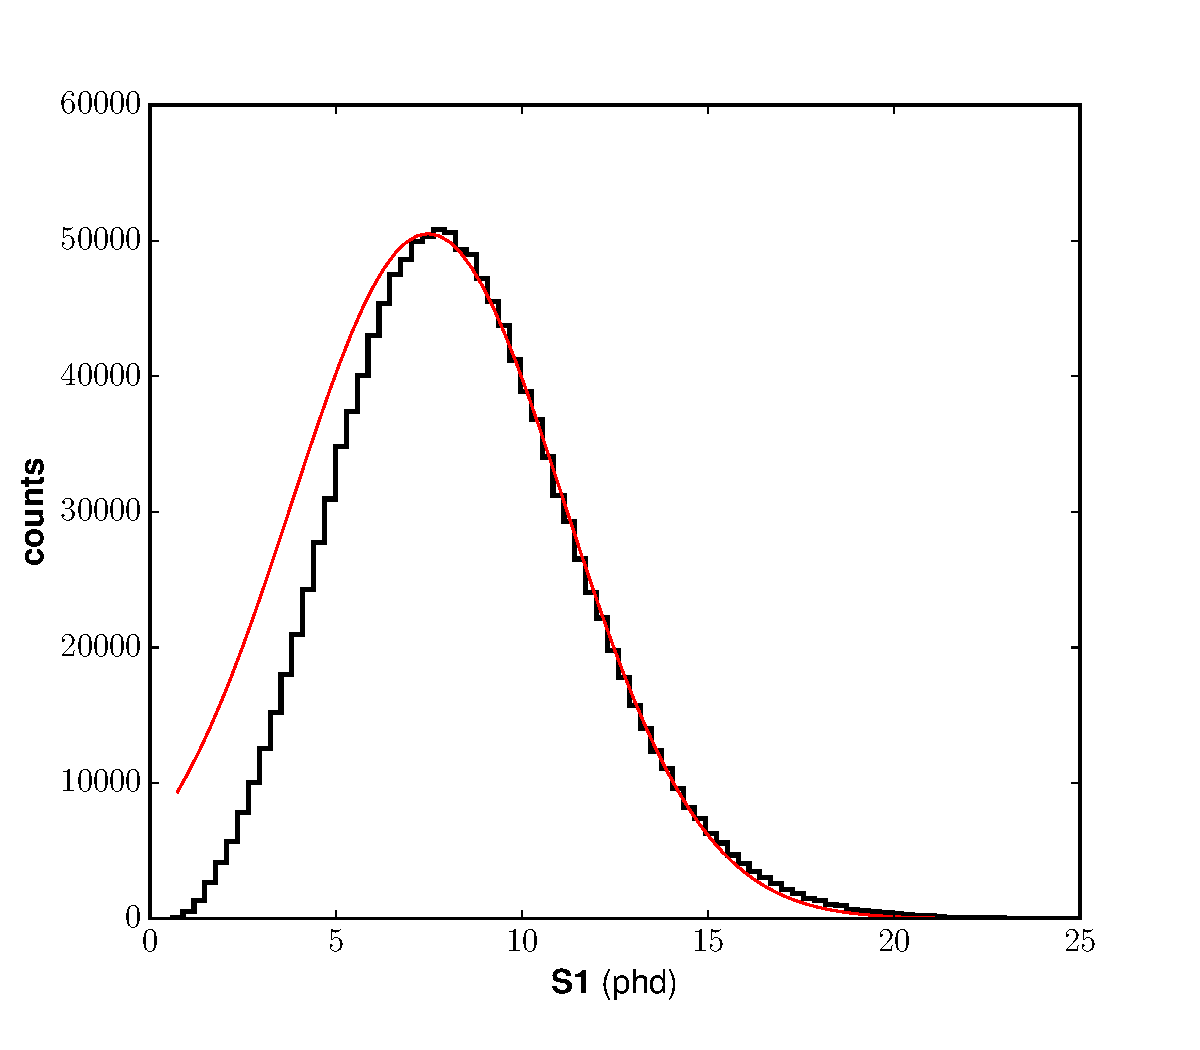
\includegraphics[width=\textwidth]{Figures/Ar37_S1spec.pdf}
  %\label{}
\end{subfigure}%
\begin{subfigure}{0.5\textwidth}
  \centering
  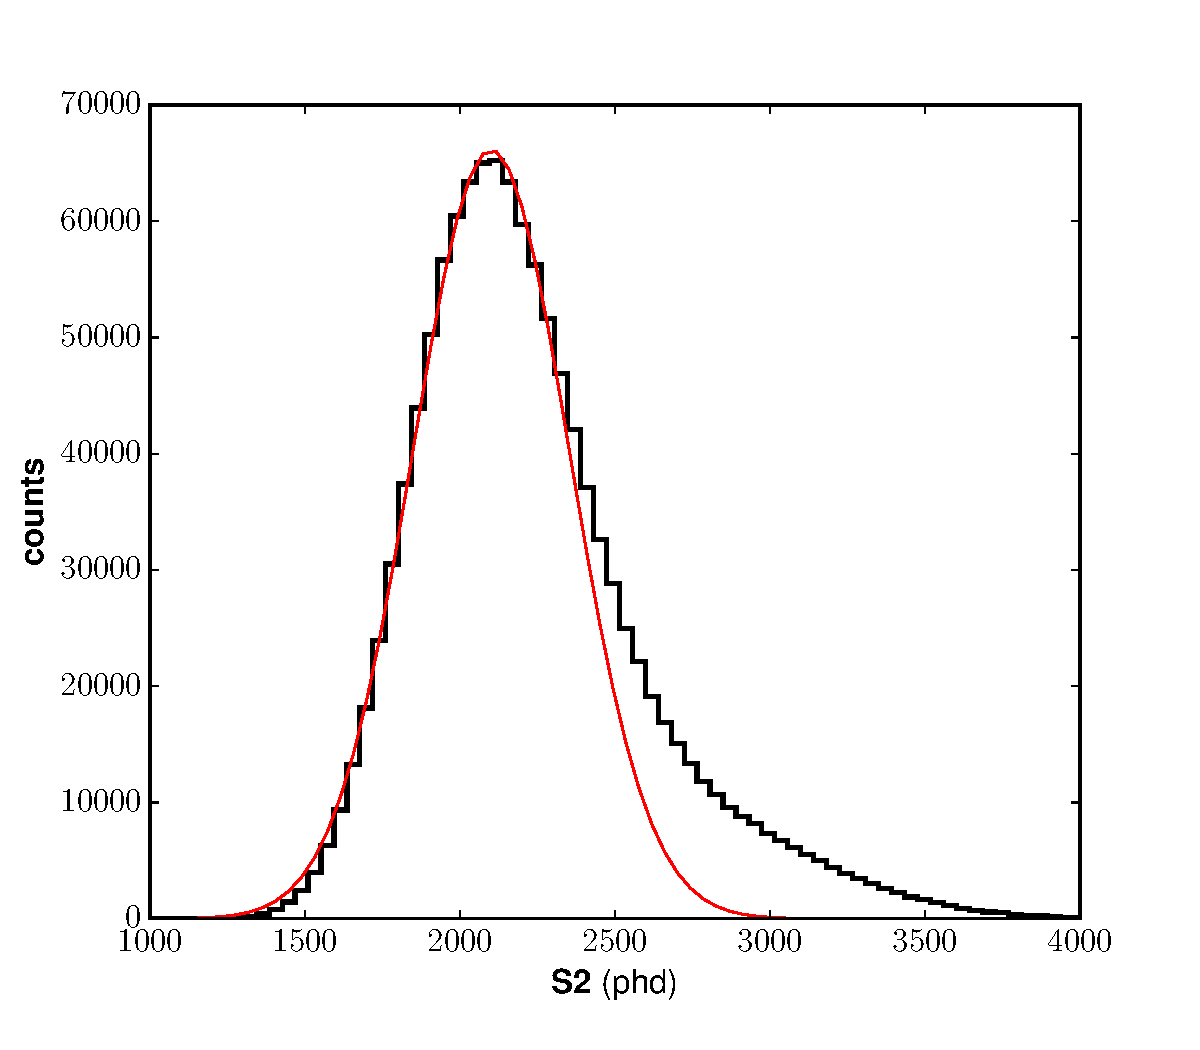
\includegraphics[width=\textwidth]{Figures/Ar37_S2spec.pdf}
  %\label{fig:intlin}
\end{subfigure}
\caption{The S1 and S2 spectra for the LUX $^{37}$Ar injection (black histograms), along with gaussian fits (red lines). Events with drift times between 105 and 170 $\mu$s. The S1 spectrum clearly does not behave like a gaussian on the low energy side of the spectrum. The S2 spectrum does have a  gaussian shape up until about 1 $\sigma$ above the mean at which point a pathological tail takes over. These S2 tails are a known issue and will be characterized in a later section.}
\label{fig:ddplot}
\end{figure}

The high rate and long lifetime of the argon-37 injection also meant that there was a huge number of events. From the injection on August 31 until the end of data-taking on September 3 there were about 8.8 million argon-37 events. The fact that we have such a high-statistics dataset, combined with the spatially uniform nature of injection sources means that we can very finely probe the position-dependence of the detector response. This feature will be used to measure the S2 efficiency corrections and in defining our radial cut.

\subsection{Radial Selection Cut}
We would like to be able to eliminate events close to the wall from our analysis. The LUX Run4 and post-Run4 drift field was highly non-uniform in the z-coordinate, so there must be a drift time dependence added to any radial event-selection cut. There is, to a lesser degree, some non-uniformity in the radial and azimuthal directions as well. Since we would like to make a radially symmetric selection cut, we can to, first order, ignore the radial dependence. The radial cut was defined by first dividing the detector into 5$\mu$s drift time bins. Each drift time bin was re-centered around the mean S2-space x and y positions. These re-centered positions were then divided into 36 $\phi$ bins. We used the assumption that the argon-37 events will be distributed uniformly in radius-squared to define the cut position for each of these $\phi$ bins. We define $r_{cut}(dT,\phi)$ such that 77\% of events in the associated bin will have $r<r_{cut}(dT,\phi)$. The true radius of this event should be $\sqrt{0.77}R_{wall}=(0.877)\cdot (25 \text{\ cm})=21.9 \text{\ cm}$. The values of $r_{cut}(dT,\phi)$ should then all be about 3 cm from the wall. We apply this cut in each drift time bin ($dT_i$) by performing a linear interpolation between the values of $r_{cut}(dT_i,\phi)$ and cutting out events with radii greater than the interpolated values.
\begin{figure}[h!]
\centering
  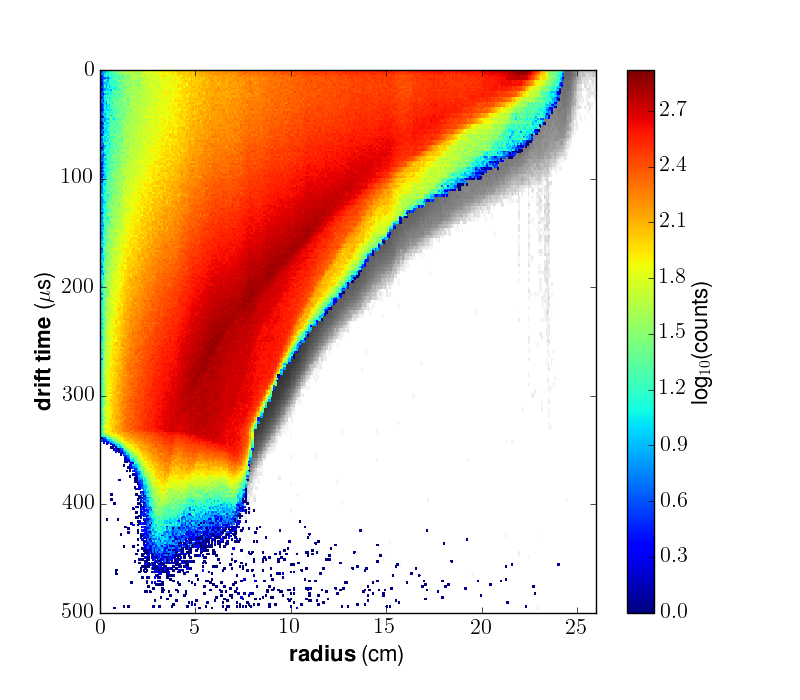
\includegraphics[width=\textwidth]{Figures/xycut_dt.png}
\caption{Visualization of the radial cut derived from the $^{37}$Ar data. The greyscale map show the data without any position cuts, while the heat-map shows the selected by the radial cuts. }
\label{fig:xycut_dt}
\end{figure}
\begin{figure}[h!]
\centering
  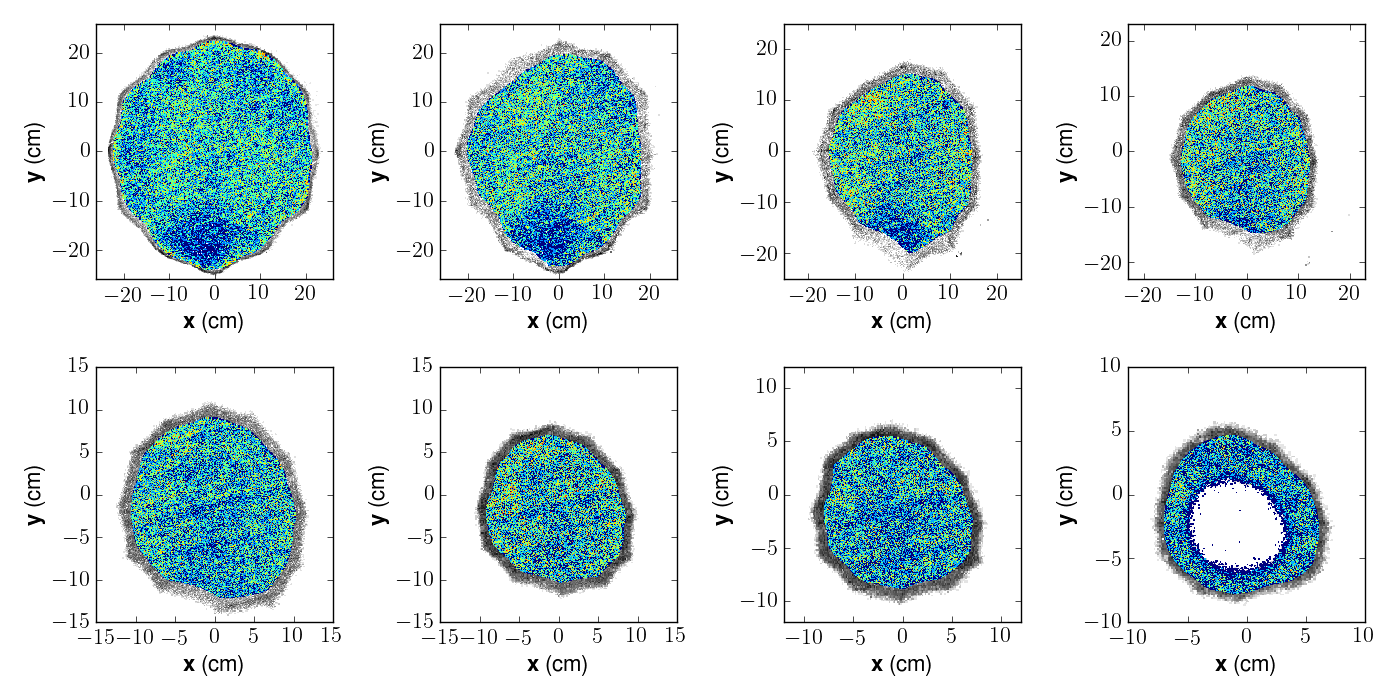
\includegraphics[width=\textwidth]{Figures/xycut_xy.png}
\caption{Selected 5 $\mu$s drift time slices used in the $^{37}$Ar drift time section cut. The greyscale map show the data without any position cuts, while the heat-map shows the selected by the radial cuts. From top left to bottom right, the drift time of the cots are 20 $\mu$s, 50 $\mu$s, 100 $\mu$s, 150 $\mu$s, 200 $\mu$s, 250 $\mu$s, 300 $\mu$s, and 350 $\mu$s. The linear diagonal lines that can be seen in the heat-maps are physical features created by the grids.}
\label{fig:xycut_xy}
\end{figure}

\subsection{S2 Efficiency Correction from $^{37}$Ar}
In Run4, the position-dependent efficiency corrections for the LUX S1 and S2 signals were obtained from a combination of tritium and $^{83m}$Kr calibration data. This method which was described in section \ref{sec:krypcal}, relies, in part, on the fact that the S2 yields for small energy deposits. The first step in the KrypCal procedure is to measure the position dependence of the tritium peak S2 value. In order to derive the detector efficiency part of the position dependence, the field effect must first be removed. This field dependence is itself dependent on the energy of the events that contribute to the S2 peak. Since tritium is a beta spectrum, events with many energies will contribute to this peak, so an approximation is made that all of these events occur at 2.5 keV.

\begin{figure}[h!]
\centering
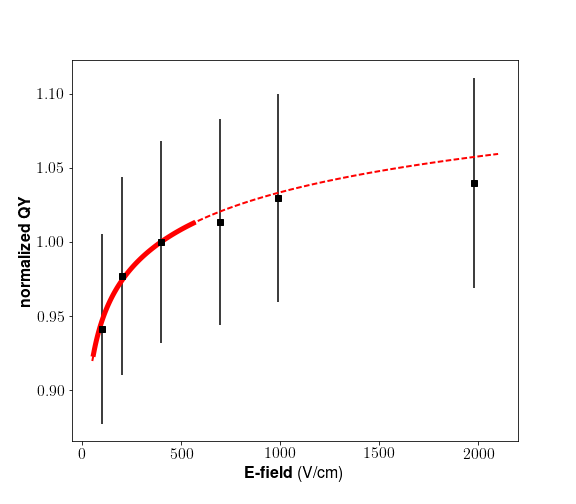
\includegraphics[width=150mm]{Figures/pixey_Ar_v_ef.png}
\caption{NEST v0.98 model of the $^{37}$Ar vs the measurements from PIXeY\cite{pixey_ar37}. The solid portion of the line indicates the range of fields in the LUX post-Run4 calibration data. There is about a 10\% variation due to electric field in the LUX post-Run4 data. The NEST v0.98 model traces the trend in the PIXeY data quite well.}
\label{fig:pixey_Ar_v_ef} 
\end{figure}
It is here that we see a huge benefit in using the $^{37}$Ar K-capture peak instead of the tritium beta spectrum in deriving the S2. Because $^{37}$Ar is a mono-energetic line source rather than a continuous beta spectrum, we know that all of the events making up the S2 peak will come from a 2.8224 keV event, and no assumption or approximation need be made. Additionally, as apposed to using a Landau function as an approximation for the S2 spectral shape, as is done for tritium, we can instead use a simple Gaussian model. 
\begin{figure}[h!]
\centering
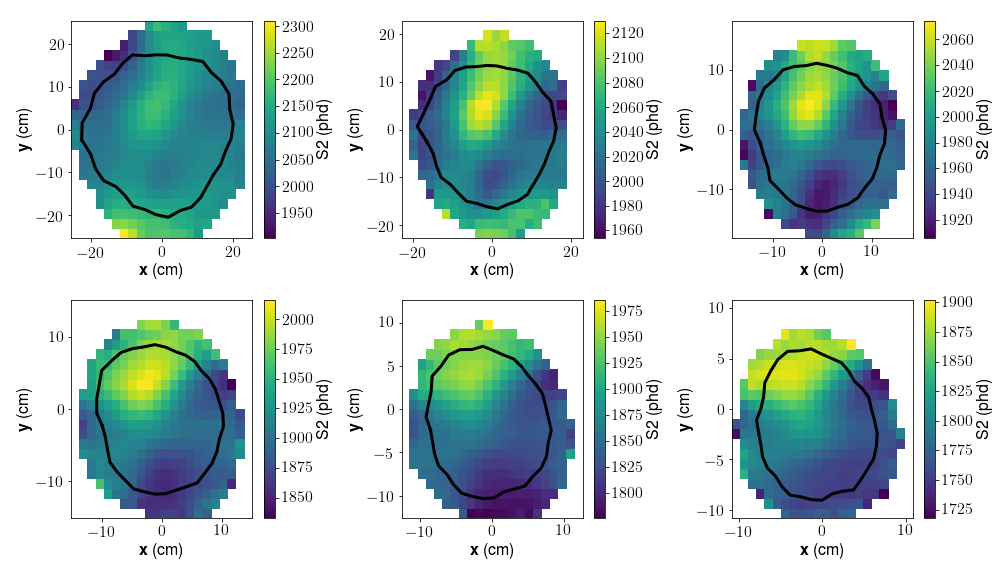
\includegraphics[width=150mm]{Figures/S2map_xy.png}
\caption{}
\label{fig:S2map_xy} 
\end{figure}

\begin{figure}[h!]
\centering
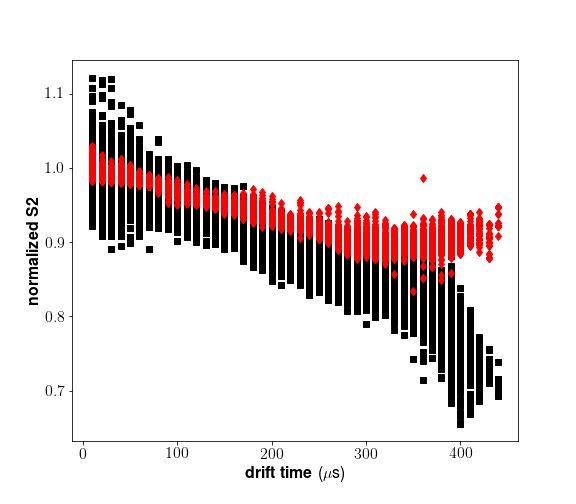
\includegraphics[width=150mm]{Figures/S2trend_dt.png}
\caption{}
\label{fig:S2trend_dt} 
\end{figure}

\begin{figure}[h!]
\centering
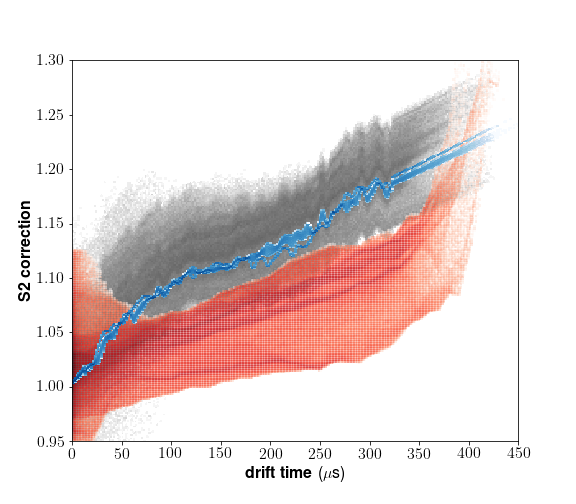
\includegraphics[width=150mm]{Figures/S2corr_dt.png}
\caption{}
\label{fig:S2corr_dt} 
\end{figure}

\begin{figure}[h!]
\centering
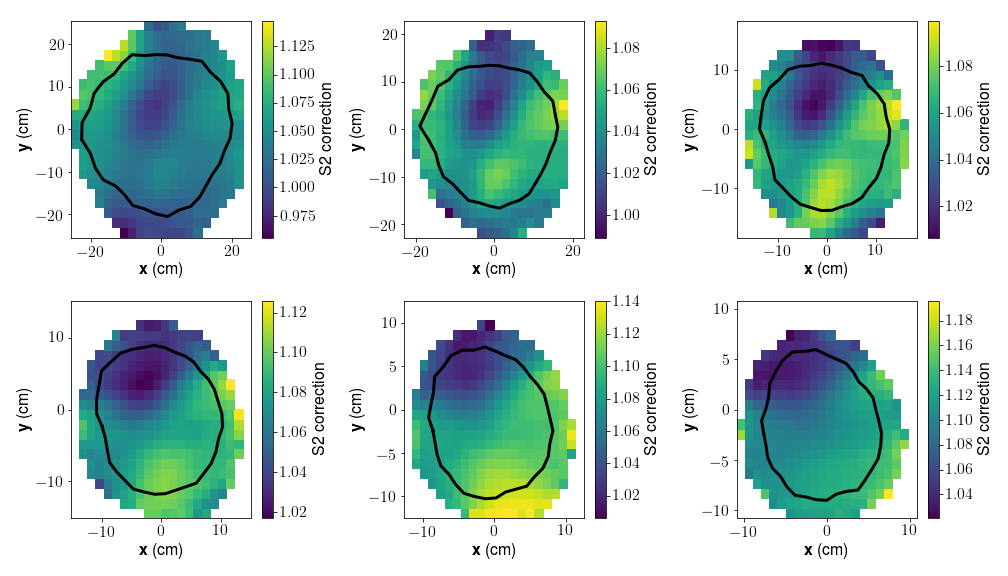
\includegraphics[width=150mm]{Figures/S2corr_xy.png}
\caption{}
\label{fig:S2corr_xy} 
\end{figure}



\section{S1 corrections from $^{131}$Xe$_{m}$+$^{83}$Kr$_{m}$ Doke Plot}
\begin{figure}[h!]
\centering
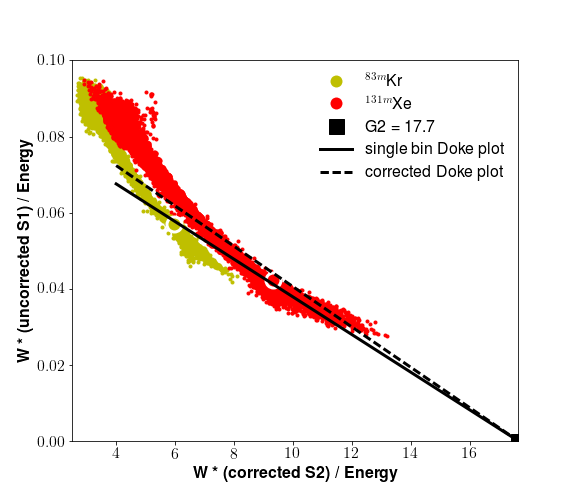
\includegraphics[width=150mm]{Figures/S1corr_singlebin.png}
\caption{}
\label{fig:S1corr_singlebin} 
\end{figure}


\begin{figure}[h!]
\centering
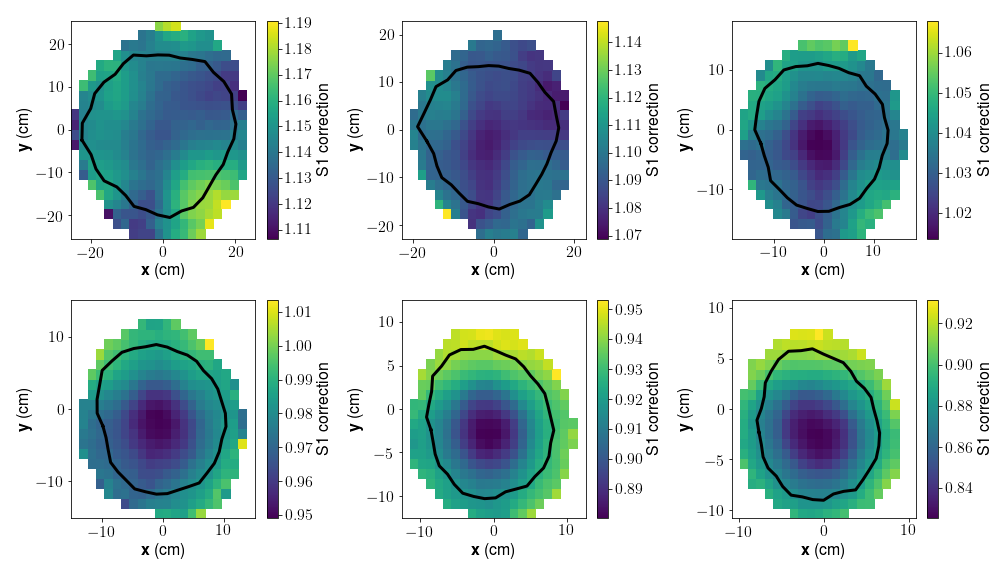
\includegraphics[width=150mm]{Figures/S1corr_xy.png}
\caption{}
\label{fig:S1corr_xy} 
\end{figure}

\begin{figure}[h!]
\centering
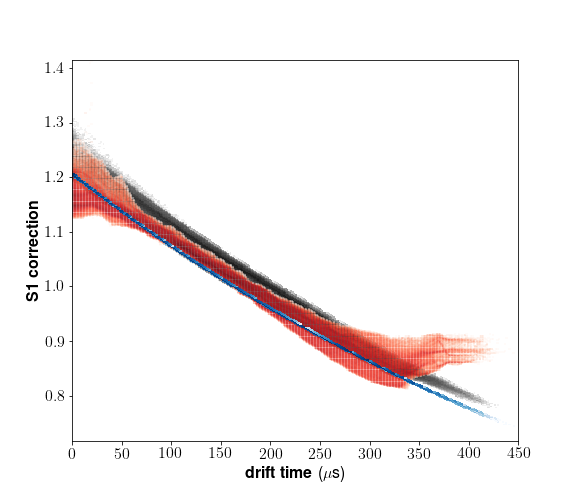
\includegraphics[width=150mm]{Figures/S1corr_dt.png}
\caption{}
\label{fig:S1corr_dt} 
\end{figure}


\begin{figure}[h!]
\centering
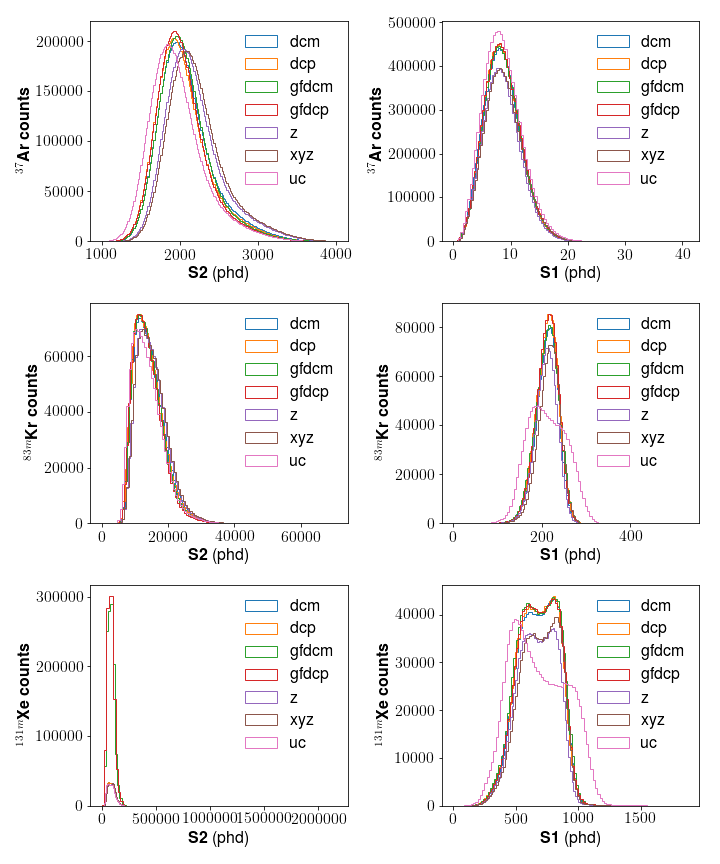
\includegraphics[width=150mm]{Figures/S1S2_spectra.png}
\caption{}
\label{fig:S1S2_spectra} 
\end{figure}


\begin{figure}[h!]
\centering
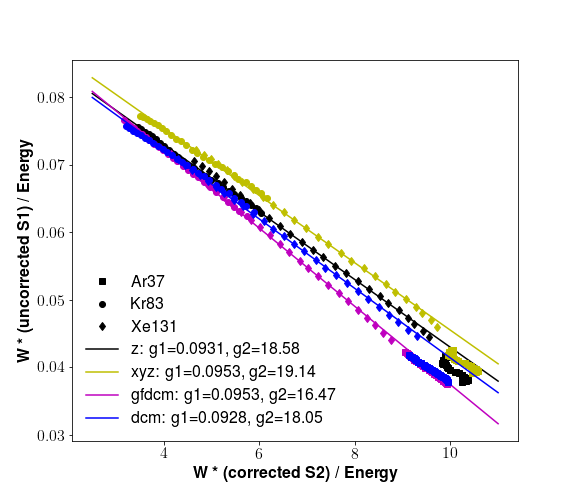
\includegraphics[width=150mm]{Figures/dt_doke_plot.png}
\caption{}
\label{fig:dt_doke_plot} 
\end{figure}

\begin{figure}[h!]
\centering
  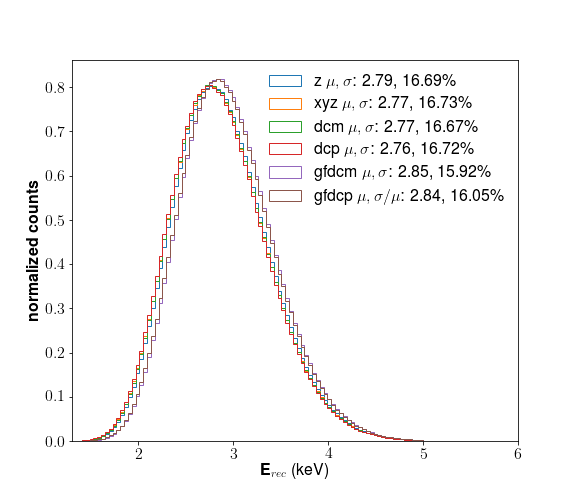
\includegraphics[width=\textwidth]{Figures/E_spec_Ar.png}
  \caption{}
\label{fig:E_spec_Ar} 
\end{figure}
  
\begin{figure}[h!]
  \centering
  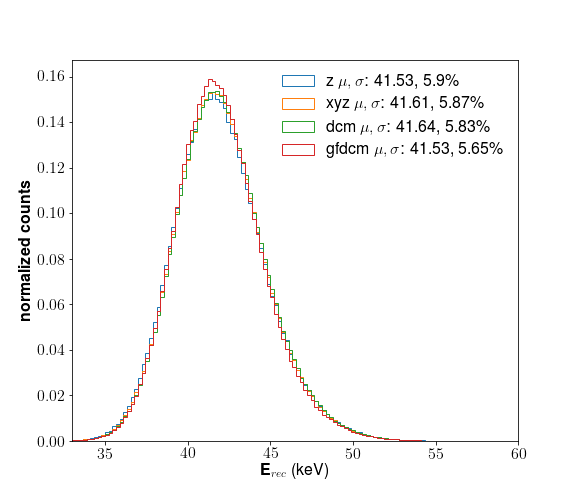
\includegraphics[width=\textwidth]{Figures/E_spec_Kr.png}
  \caption{}
\label{fig:E_spec_Kr} 
\end{figure}

  
\begin{figure}[h!]
  \centering
  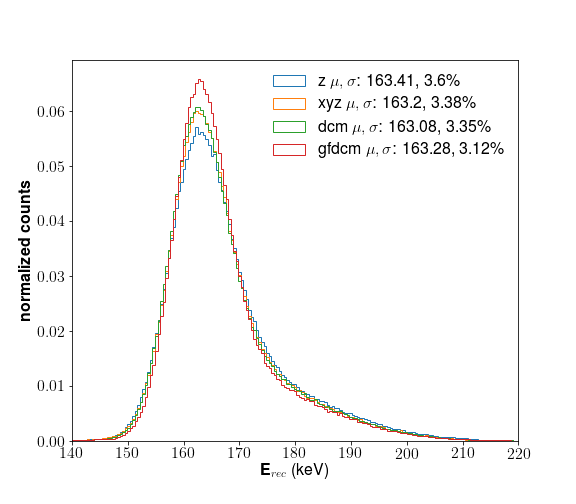
\includegraphics[width=\textwidth]{Figures/E_spec_Xe.png}
  \caption{}
\label{fig:E_spec_Xe} 
\end{figure}


\section{CH$_{3}$T Calibrations}


\subsection{Model of Pathological S2 Tails derived from $^{131}$Xe$_{m}$ and Tritium}

\begin{figure}[h!]
\centering
\begin{subfigure}{0.5\textwidth}
  \centering
  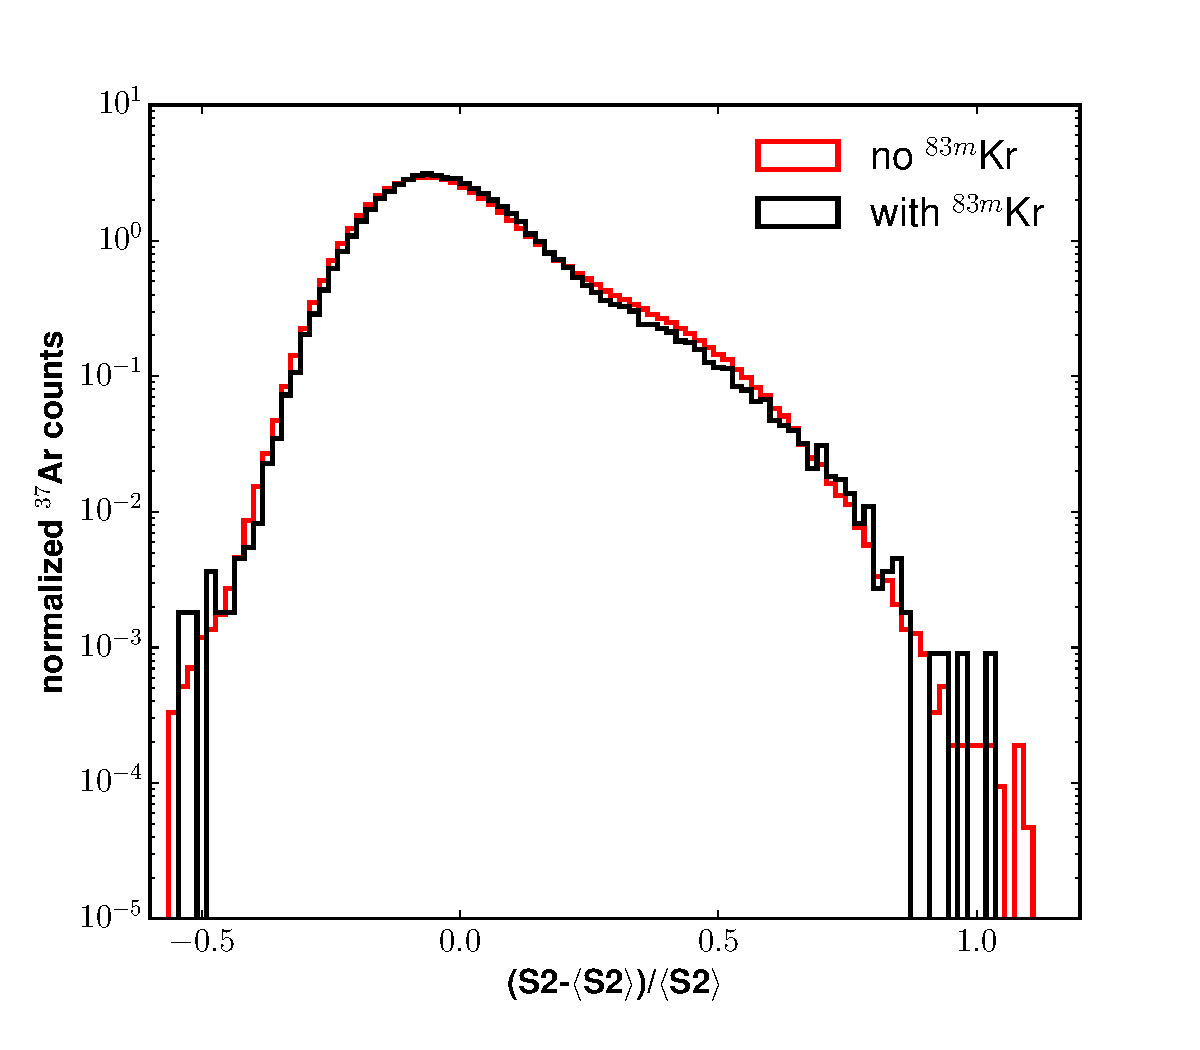
\includegraphics[width=\textwidth]{Figures/S2_tail_spec_Ar_rate.pdf}
  \caption{}
\end{subfigure}%
\centering
\begin{subfigure}{0.5\textwidth}
  \centering
  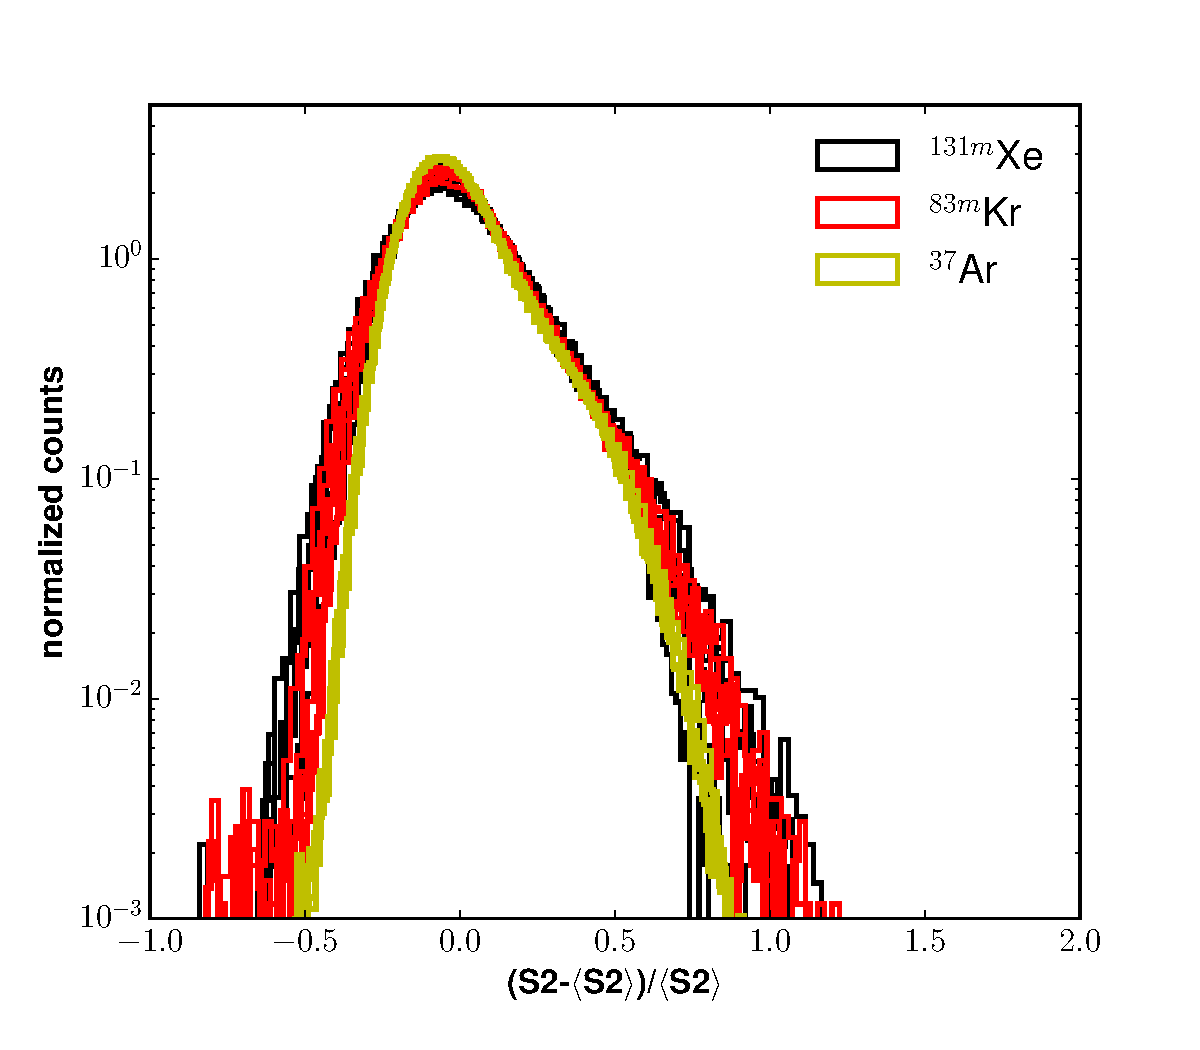
\includegraphics[width=\textwidth]{Figures/S2_tail_spec_all.pdf}
  \caption{}
\end{subfigure}
\caption{}
\label{fig:S2_tail_specl} 
\end{figure}


\section{$^{14}$CH$_4$ Injection}






